\documentclass[tikz,border=10pt]{standalone}
\begin{document}
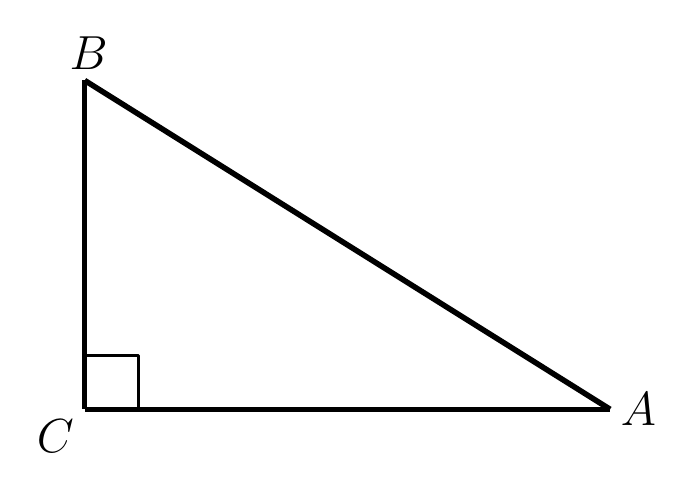
\begin{tikzpicture}[line join=round, line width=1.2pt]
% Coordinates: C at origin, s = 0.021277 cm/px, y axis flipped (up = +y)
\coordinate (C) at (0,0);
\coordinate (A) at (6.672,0);   % A: dx=313.6 px
\coordinate (B) at (0,4.176);   % B: dy=196.25 px
% Right-angle mark at C (side 21.52 px = 0.458 cm), arms toward A (+x) and B (+y)
\coordinate (Mx) at (0.68700000000000,0.00000000000000);
\coordinate (Mxy) at (0.68700000000000,0.68700000000000);
\coordinate (My) at (0.00000000000000,0.68700000000000);

% Triangle sides AB, BC, CA (solid, no fill), stroke raised to 2pt
\draw[line width=2pt] (A) -- (B);
\draw[line width=2pt] (B) -- (C);
\draw[line width=2pt] (C) -- (A);

% Single right-angle square mark at C
\draw (Mx) -- (Mxy) -- (My);

% Labels (font from style metrics); B nudged right: sits above and slightly right of vertex
\node[right] at (A) {\fontsize{17.5}{21}\selectfont $A$};
\node[anchor=south, xshift=0.05cm] at (B) {\fontsize{17.5}{21}\selectfont $B$};
\node[below left] at (C) {\fontsize{17.5}{21}\selectfont $C$};
\end{tikzpicture}
\end{document}